\documentclass[lettersize,journal]{IEEEtran}
\usepackage{amsmath,amsfonts}
\usepackage{algorithmic}
\usepackage{algorithm}
\usepackage{array}
\usepackage[caption=false,font=normalsize,labelfont=sf,textfont=sf]{subfig}
\usepackage{textcomp}
\usepackage{stfloats}
\usepackage{url}
\usepackage{verbatim}
\usepackage{graphicx}
\usepackage{cite}
\hyphenation{op-tical net-works semi-conduc-tor IEEE-Xplore}
% updated with editorial comments 8/9/2021

\begin{document}

\title{Visual Prompting in Vision-Language Models for Multi-Face Emotion Recognition: Reproducing and Extending Set-of-Vision}

\author{Badagoni Sri Sahasra, B24DS003}

\maketitle

\section{Project Details}
\textbf{Criterion followed:} reproduce paper results (and extend them). We reproduce the Set-of-Vision (SoV) visual-prompting study of Zhang et al.~\cite{zhang2024visual}, replacing the closed GPT-4V with open vision-language models, and we add the extensions listed in Section~\ref{sec:lim}.

Team composition and individual contributions (solo project):
\begin{itemize}
    \item Member 1: Badagoni Sri Sahasra, B24DS003, badagonisrisahasra@gmail.com. Entire project: dataset preparation, face detection and labelling, visual-prompt rendering, model inference, evaluation, analysis and report.
\end{itemize}
Code: \url{https://github.com/sahasraa19/soV-emotion-recognition}

\section{Problem Statement}
Vision-language models (VLMs) can describe a face's emotion, but with many faces in one image they confuse which face the question refers to. SoV prompting~\cite{zhang2024visual} addresses this by drawing cues on the image before asking the question: bounding boxes, a number tag per face and five facial landmarks. The question then refers to ``face 3'' instead of a position in the picture.

\textbf{Motivation.} Emotion recognition in groups (classrooms, meetings, crowds) needs several faces handled at once, and visual prompting needs no training. It is important to know which cues really help and which hurt, and whether the result holds for small open models.

\textbf{Scope.} Zero-shot emotion recognition (7 classes: angry, disgust, fear, happy, sad, surprise, neutral) on multi-face images, comparing 10 visual-prompt variants. We do not train any model.

\section{Methodology}
\textbf{Models.} Qwen2-VL-7B-Instruct~\cite{wang2024qwen2vl} (4-bit, greedy decoding) is the main model; LLaVA-1.5-7B~\cite{liu2024improved} is the second model. Both are used zero-shot.

\textbf{Pipeline} (Fig.~\ref{fig_1}): (1) prepare images; (2) detect faces with RetinaFace~\cite{deng2020retinaface} (YuNet fallback), drop faces under 32 px, remove overlapping boxes (paper Algorithm 1, threshold 0.5) and number faces left to right; (3) obtain ground-truth emotions; (4) render the visual prompt; (5) ask one fixed question that returns JSON with the face count and one emotion per face; (6) evaluate.

\textbf{Visual-prompt variants.} V0 plain image; V1 RedCircle-style~\cite{shtedritski2023redcircle}; V2 ReCLIP-style~\cite{subramanian2022reclip}; V3 boxes; V4 boxes+numbers; V5 full SoV (boxes+numbers+landmarks); V6 numbers only; V7 landmarks only; V8, V9 = V5, V7 with much smaller landmark dots (our extension).

\textbf{Metrics.} Per-face accuracy, macro precision/recall/F1, face-count accuracy, majority-class baseline, and 95\% bootstrap confidence intervals over images for the difference to the plain image. Numbered variants are matched to ground truth by the number tag; others by left-to-right position.

\textbf{Difference from existing work.} The original study used GPT-4V and its own 119 images. We use open models, a fixed standardized prompt for all variants, confidence intervals, and a modular, re-runnable code base (\texttt{src/} modules, one script per stage).

\begin{figure}[!t]
\centering
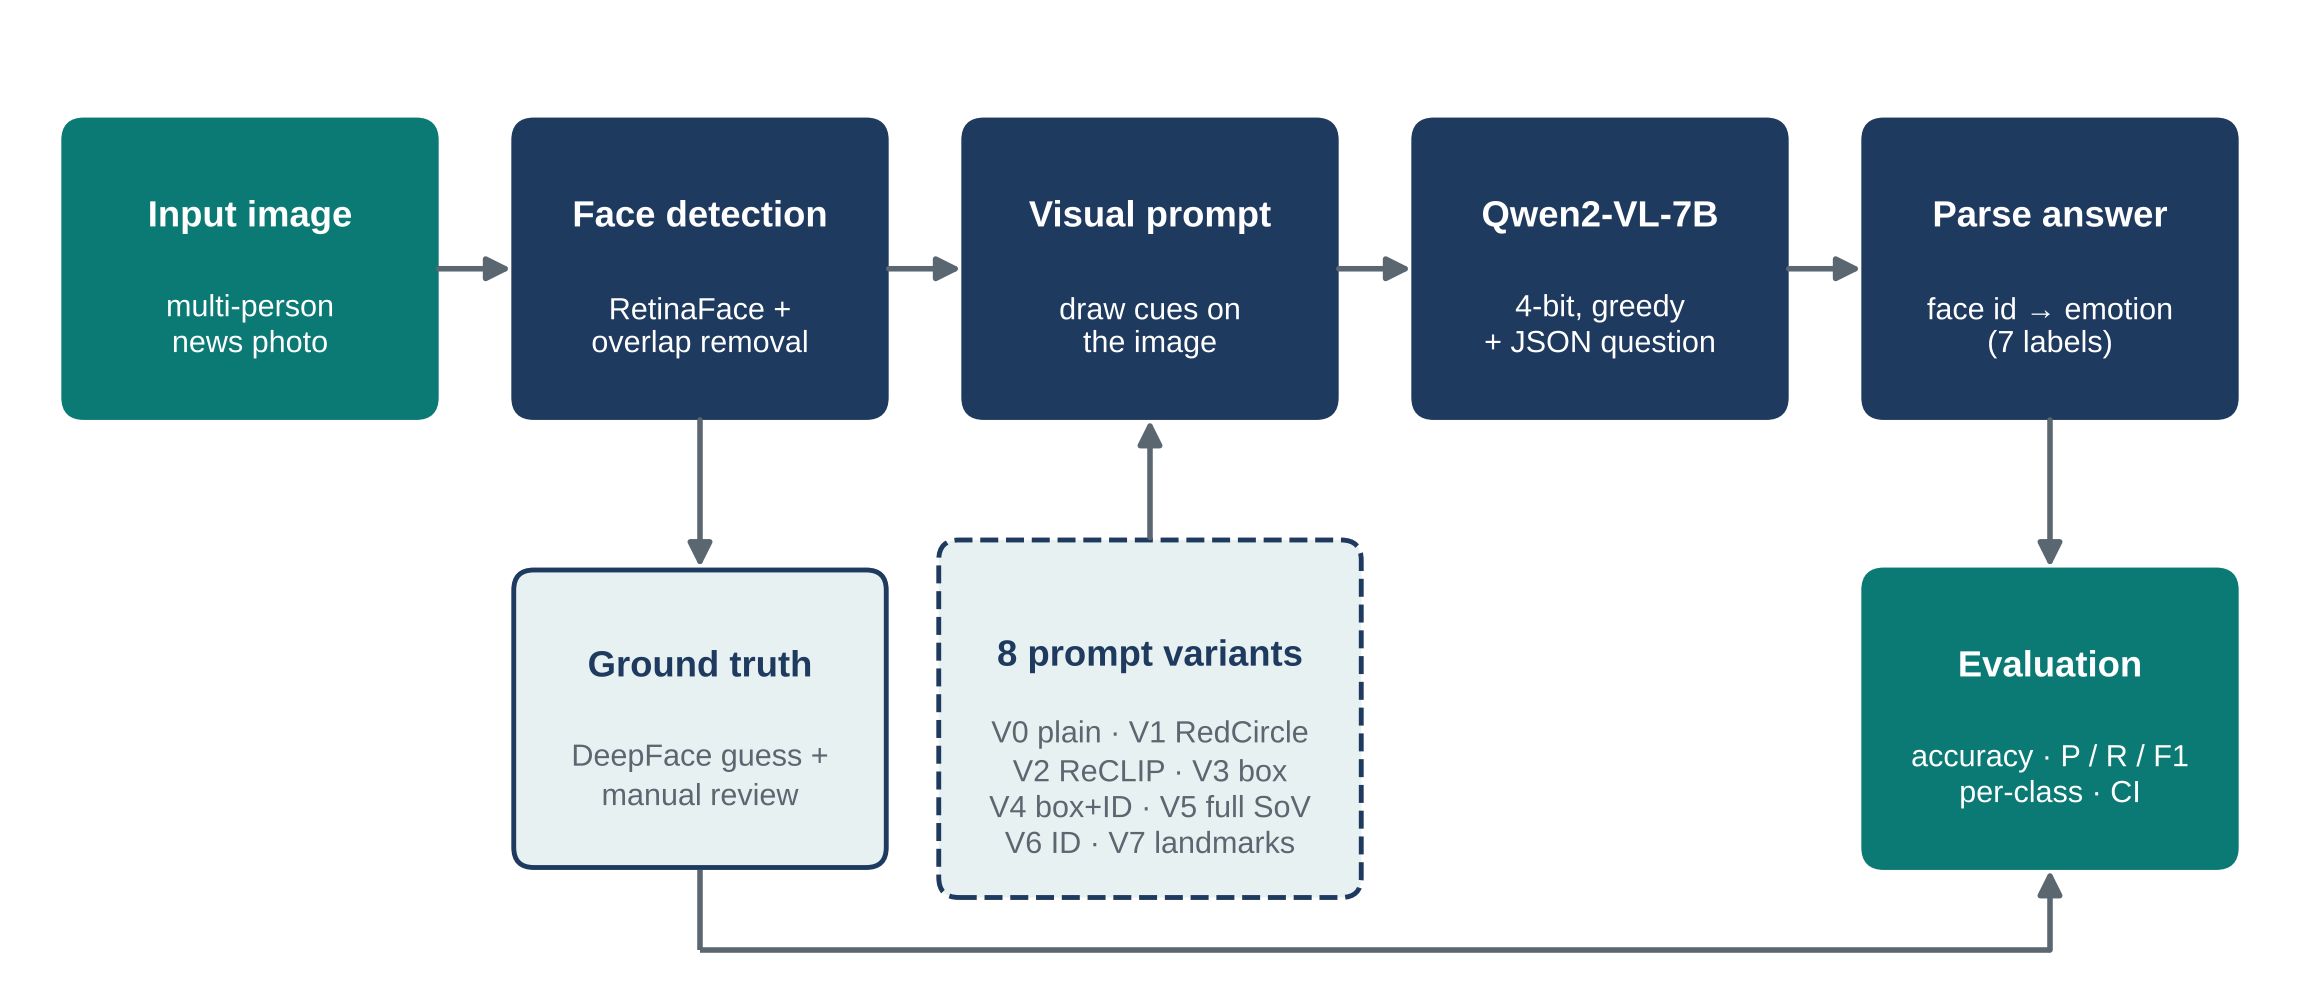
\includegraphics[width=3.3in]{fig1}
\caption{Pipeline of the proposed system.}
\label{fig_1}
\end{figure}

\section{Resource and Dataset Availability}
\textbf{Phase 1 data (own photos).} 17 group photos, 77 faces (neutral 27, happy 24, sad 15, angry 6, fear 2, surprise 2, disgust 1). Labels: DeepFace first guess followed by manual correction. Majority-class baseline is 35.1\%.

\textbf{Phase 2 data.} FER-2013~\cite{goodfellow2013fer} provides emotion-labelled 48$\times$48 faces; WIDER FACE~\cite{yang2016wider} provides real crowd photos. We sample a class-balanced set of FER-2013 test faces (20 per emotion in the current build, 140 faces) and place 2 to 8 of them on a blurred WIDER photo, giving 60 images with 302 faces. Boxes, landmarks and labels are known exactly, so no manual labelling is needed. WIDER is used only as background, because the annotation file was not used. FER-2013 labels are noisy (human agreement is about 65\%), so absolute accuracy is limited by label quality.

\textbf{Resources.} Google Colab T4 GPU (16 GB) with 4-bit quantisation; Python, PyTorch, Transformers, bitsandbytes, OpenCV, DeepFace, scikit-learn, matplotlib. No paid API is required.

\section{Limitations Found}
\label{sec:lim}
\textbf{Observed in Phase 1 (Qwen2-VL-7B, real results).} Table~\ref{tab:table1} shows accuracy. Only the RedCircle-style variant clearly helped (+6.5 points, CI +1.1 to +12.9). Full SoV (V5) was 5.2 points below plain (CI $-19.3$ to $+6.0$, not clearly different) and answered ``neutral'' for 82\% of faces. Landmarks only (V7) was 11.7 points worse (CI $-26.0$ to $-1.1$). Number tags gave 100\% face-count accuracy against 94.1\% for plain. So the paper's claim that full SoV helps was not reproduced on this small open model; the dots are large and may cover the eyes and mouth.

\textbf{How we address it.} (i) V8/V9 repeat the landmark cues with small dots; (ii) a second model (LLaVA-1.5-7B) checks whether the finding is model-specific; (iii) a larger test set (Phase 2) reduces the wide confidence intervals of 77 faces; (iv) one standardized prompt for every variant.

\textbf{Limitations of our work.} Small Phase 1 sample; FER-2013 labels are noisy and its faces are low-resolution; Phase 2 faces are pasted, not natural scenes; each FER face is reused about twice; one model decoding setting. \emph{Status: the Phase 2 model runs (Qwen2-VL and LLaVA on the 60 composite images) and the V8/V9 results are not finished at the time of writing, so no results are reported for them.}

\begin{table}[!t]
\caption{Phase 1: Qwen2-VL-7B accuracy on 77 faces (majority class 35.1\%).\label{tab:table1}}
\centering
\begin{tabular}{|l|c|c|}
\hline
Variant & Accuracy \% & Face-count \% \\
\hline
V0 Plain & 46.8 & 94.1 \\
V1 RedCircle & 53.2 & 88.2 \\
V2 ReCLIP & 42.9 & 88.2 \\
V3 Boxes & 42.9 & 88.2 \\
V4 Boxes+numbers & 49.4 & 100 \\
V5 Full SoV & 41.6 & 100 \\
V6 Numbers only & 48.1 & 100 \\
V7 Landmarks only & 35.1 & 94.1 \\
\hline
\end{tabular}
\end{table}

\section{Expected Outcomes}
\begin{itemize}
    \item Complete the Phase 2 runs for both models and report accuracy, macro recall and confidence intervals for all 10 variants, plus the SoV-minus-plain difference per model.
    \item Show whether small dots (V8/V9) recover the loss seen with large dots.
    \item Final outputs: modular open-source repository with scripts, notebooks, saved raw outputs and analysis folders; this report.
\end{itemize}

\nocite{lecun2015deep}
\nocite{vaswani2017attention}

\bibliographystyle{IEEEtran}
\bibliography{ref}

{\appendix
\textbf{Platforms and prompts.} Google Colab (T4 GPU) for model inference; Python with Hugging Face Transformers for Qwen2-VL-7B-Instruct and LLaVA-1.5-7B; Claude (Anthropic) was used as an assistant for code structuring, debugging, and drafting this report. The model prompt (the same for all variants except one sentence describing the drawing) is: ``You are an expert in facial expression analysis. Task: (1) count the human faces that are clearly visible in the image and (2) classify the facial emotion of every one of those faces. Allowed labels: angry, disgust, fear, happy, sad, surprise, neutral. [variant sentence] Answer ONLY with JSON: \{num\_faces, faces:[\{id, emotion\}]\}.''}

\end{document}
